\section{Optimálne zastavenie DC motora}

DC motor je často využívaným zariadením v priemysle, ale aj v bežnom živote. Môže nadobúdať rôzne veľkosti a formy a jeho účelom je meniť elektrickú energiu na energiu mechanickú. Čo je pre nás dôležité, pracuje pod veľmi malou periódou vzorkovania. Je to teda systém s veľmi rýchlou dynamikou a nedá sa jednoducho riadiť pomocou nelineárneho MPC. 
\label{math:model_DC}
V tomto prípade budeme mať model systému opísaný nelineárnymi diferenciálnymi rovnicami, ktoré sú v nasledovnom tvare
\begin{align}
& \dot{x}_1(t) = - \frac{R}{L_{a}}x_1(t) - \frac{k_{m}}{L_{a}}u(t)x_{2}(t) + \frac{u_a}{L_a}\\
& \dot{x}_2(t) = - \frac{B}{J}x_2(t) - \frac{k_{m}}{J}u(t)x_{1}(t) + \frac{\tau_l}{J}\\
& y(t) = x_{1}(t)
\end{align}
kde prvý stav $x_{1}$ predstavuje prúd rotora v $[A]$, druhý stav $x_{2}$ predstavuje uhlovú rýchlosť v $[rad/s]$ a vstupom $u$ je prúd statora udávaný v $[A]$. Naša sledovaná veličina bude uhlová rýchlosť (druhý stav)\cite{bib2}.
\begin{table}[h!]
	\centering
	\caption{Parametre DC motora \cite{bib2}}
	\label{tab.1: Parametre DC motora}
	\begin{tabular}{c c c}
		\hline
		\textbf{Značka} & \textbf{Hodnota} & \textbf{Veličina} \\ \hline
		$L_{a}$ & $0,314$ & $H$ \\ 
		$R_{a}$ & $12,345$ & $\Omega$ \\ 
		$k_{m}$ & $0,253$ & $N m A^{-2}$ \\ 
		$J$ & $0,00441$ & $N m s^{-2}$ \\ 
		$B_{a}$ & $ 0,00732$ & $N m s$ \\ 
		$\tau_l$ & $1,47$ & $N m$ \\
		$u_{a}$ & $60$ & $V$ \\ \hline
	\end{tabular}
\end{table}

Keďže máme model v kontinuálnej časovej oblasti musíme si ho pretransformovať do diskrétnej podoby. Využijeme pri tom Euilerovú metódu, kde aproximujeme kontinuálny model diskrétnym podľa teórie, ktorú sem si uvideli v kapitole \hyperref[se:diskretizacia]{Euilerova metóda diskretizácie (2.2)}. Model systému po diskretizácií má nasledovnú podobu
\begin{align}
& x_{k+1}^{1} = x^{1}_{k}+T_{s}\left(- \frac{R}{L_{a}}x^{1}_{k} - \frac{k_{m}}{L_{a}}u_{k}x^{2}_{k} + \frac{u_a}{L_a}\right)\\
& x_{k+1}^{2} = x^{2}_{k}+T_{s}\left(- \frac{B}{J}x^{2}_{k} - \frac{k_{m}}{J}u_{k}x^{1}_{k} + \frac{\tau_l}{J}\right)\\
& y(t) = x^{1}_{k}
\end{align}
kde $T_{s}$ je perióda vzorkovania , ktorú sme použili ako krok diskreditácie. Keďže sa jedná o veľmi rýchly systém jeho perióda vzorkovania je preto veľmi malá v našom prípade je to $T_{s} = 50ms$. Túto periódu musíme počas riadenia dodržal ak chceme aby náš prediktívny regulátor bol stabilný a stihol vypočítať akčný zásah v každej perióde.

Našou úlohou je čo najefektívnejšie zastaviť DC motor z referenčných stavov, $x_{0}^{1}=0,887 A$ a $x_{0}^{2}=0,587 s^{-1}$ pričom nás fyzikálne obmedzuje vstup do systému $-4 \leq u_{k} \leq 4$. 

Ako prvé si zadefinujeme nelineárne MPC s ohraničeniami ($N = 5$), vo forme ktorú sme si ukázali v kapitole  \hyperref[subse:NelinearneMPC]{Nelineárne riadenie (2.1.3)}. Pomocou logaritmickej bariéry si môžeme pridať ohraničenia do účelovej funkcie a vytvoríme si tak neohraničený optimalizačný problém, bližšie si môžeme pozrieť kapitolu \hyperref[subse:Ohranicenia]{Ohraničené riadenie (2.4.3)}. Ďalej len riešime problém bez ohraničení ako sme popísali v časti \hyperref[subse:Nelin_MPC_ADMM]{Nelineárne prediktívne riadenie pomocou ADMM (2.4.2)}, rozdistribuujeme si MPC na $N$ predikčných horizontov, pridáme duálne funkcie a vytvoríme si rozšírený lagrangean. Rovnako ako v predošlej simulácií, kritériá pre zastavenie \hyperref[subse:ADMM2]{iterácií v ADMM} sme zvolili presnosť hľadaných počiatočných stavov $\norm{x_{k}(x_{k-1},u_{k-1})- x_{k}} < \epsilon,\hspace{0.5cm} k=1,\dots,N-1$ a taktiež veľkosť zmeny predikovaných akčných zásahov $\norm{u{k}^{i-1}-u{k}^{i}} < \epsilon,\hspace{0.5cm} k=0,\dots,N-1$, kde $\epsilon = 1\mathrm{e}{-5}$. Pre porovnanie výsledkov normálneho MPC a decentralizovaného MPC sme vytvorili simuláciu na nelineárnom modely, \hyperref[math:model_DC]{rovnice (3.5,3.6)}.
\begin{figure}[H]
	\centering
	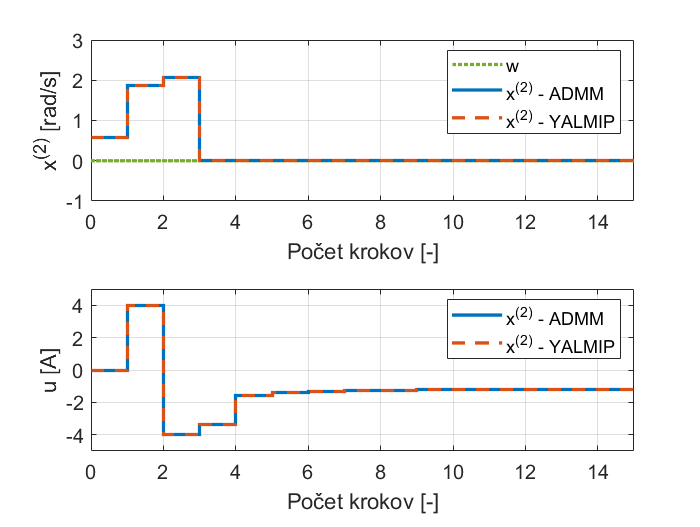
\includegraphics[width=13cm,height=10cm]{images/DC_motor/Priebeh_riadenia_a_akcne_zasahy}
	\caption{Priebeh riadenia DC motora}
	\label{fig7: PR}
\end{figure}
Ako môžeme vidieť na (Obr 3.4) v oboch prípadoch sa nám podarilo dosiahnuť žiadanú veličinu s totožným priebehom riadenia. 
\newpage
\begin{figure}[H]	
	\centering
	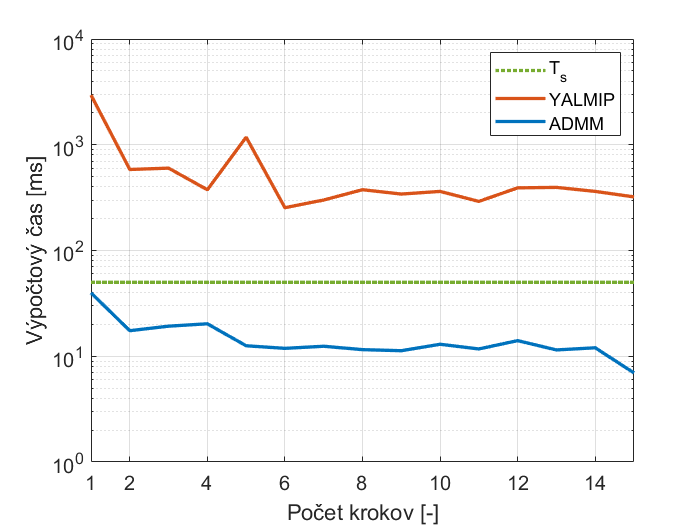
\includegraphics[width=13cm,height=10cm]{images/DC_motor/Vypoctovy_cas}
	\caption{Porovnanie výpočtovej náročnosti MPC, medzi ADMM a YALMIP}
	\label{fig9: VN}
\end{figure}
Na (Obr. 3.5) si môžeme všimnúť, že pomocou analistického riešiteľa z toolboxu YALMIP sme sa ani len nepriblížili k perióde vzorkovania DC motora a preto nieje možné používať takýto spôsob výpočtu MPC pre riadenie takéhoto systému. Naopak pomocou ADMM sa nám podarilo dosiahnuť veľmi dobré výsledky. Vďaka ADMM sme mohli rozdeliť jeden optimalizačný problém na päť decentralizovaných a riešiť ich samostatne. Takéto rozdelenie zmenšilo počet iterácií v Newtonovej numerickej optimalizácií a zároveň umožnilo paralelné riešenie týchto decentralizovaných problémov. Vo výsledku vidíme, že sa nám podarilo dostatočne zrýchliť výpočet akčných zásahov a stíhame ich opakovane počítať v rámci periódy vzorkovania $T_{s} = 50ms$.